\documentclass[10pt]{beamer}

\usepackage[brazilian]{babel}
\usepackage[utf8]{inputenc}
\usepackage[T1]{fontenc}
\usepackage{listings}
\usepackage{graphicx}
\usepackage[utf8]{inputenc}
\usepackage[T1]{fontenc}
\usepackage{helvet}

\usetheme[left]{AAUsidebar}
% colored hyperlinks
\newcommand{\chref}[2]{%
  \href{#1}{{\usebeamercolor[bg]{AAUsidebar}#2}}%
}

\title[Java SWING]% optional, use only with long paper titles
{\textbf{Java SWING}}

\subtitle{MATA55 - Programação Orientada a Objetos}  % could also be a conference name

\author[Frederico Durão] % optional, use only with lots of authors
{
  Profº Frederico Durão\\
  \href{mailto:freddurao@dcc.ufba.br}{{\tt freddurao@dcc.ufba.br}}
}

\institute[
  {
\includegraphics[scale=0.2]{AAUgraphics/logodcc}}\\ %insert a company, department or university logo
%  Dept.\ de Ciência da Computação\\
 % UFBA\\

] % optional - is placed in the bottom of the sidebar on every slide
{% is placed on the title page
  Instituto de Matemática\\
  Departamento de Ciência da Computação\\
  Universidade Federal da Bahia\\

  
  %there must be an empty line above this line - otherwise some unwanted space is added between the university and the country (I do not know why;( )
}


% specify a logo on the titlepage (you can specify additional logos an include them in 
% institute command below
\pgfdeclareimage[height=3cm]{titlepagelogo}{AAUgraphics/aau_logo_new} % placed on the title page
%\pgfdeclareimage[height=1.5cm]{titlepagelogo2}{graphics/aau_logo_new} % placed on the title page
\titlegraphic{% is placed on the bottom of the title page
  \pgfuseimage{titlepagelogo}
%  \hspace{1cm}\pgfuseimage{titlepagelogo2}
}

% Formatação dos trechos em Java
\definecolor{dkgreen}{rgb}{0,0.6,0}
\definecolor{gray}{rgb}{0.5,0.5,0.5}
\definecolor{mauve}{rgb}{0.58,0,0.82}

\lstset{frame=tb,
  language=Java,
  aboveskip=3mm,
  belowskip=3mm,
  showstringspaces=false,
  columns=flexible,
  basicstyle={\small\ttfamily},
  numbers=none,
  numberstyle=\tiny\color{gray},
  keywordstyle=\color{blue},
  commentstyle=\color{dkgreen},
  stringstyle=\color{mauve},
  breaklines=true,
  breakatwhitespace=true
  tabsize=3
}
%Formatação dos trechos em java acabam aqui.



\begin{document}
% the titlepage
{\aauwavesbg%
\begin{frame}[plain,noframenumbering] % the plain option removes the sidebar and header from the title page
  \titlepage
\end{frame}}
%%%%%%%%%%%%%%%%

% TOC
\begin{frame}[allowframebreaks]{Agenda}{}
\tableofcontents{}
\end{frame}
%%%%%%%%%%%%%%%%

\section{Introdução}
\subsection{O que é Java Swing}
\begin{frame}{Introdução}{O que é Java Swing}
\begin{itemize}
\item Swing é uma API Java para interfaces gráficas. 
\item Faz parte da JFC (Java Foundation Classes) que encapsula um grupo de 'features' para GUIs (Graphical User Interfaces).
\end{itemize}
\end{frame}
\subsection{Por que estudar Java Swing}
\begin{frame}{Introdução}{Por que estudar Java Swing}
\end{frame}
\subsubsection{Swing vs. others}
\begin{frame}{Introdução}{Por que estudar Java Swing}{Swing vs. others}
\end{frame}
%			EXT-GWT
%			Android
%			JSF + PrimeFaces
%			OpenGL, WebGL
\subsection{Como usar o Java Swing}
\begin{frame}{Introdução}{Como usar o Java Swing}
\begin{itemize}
\item Editor convencional.
\item Plugins Drop \& Drag.
\end{itemize}
\end{frame}{}
\subsubsection{Codificando no Editor convencional}
\begin{frame}{Introdução}{Como usar o Java Swing}{Codificando no Editor convencional}
\lstinputlisting[language=Java]{codes/HelloWorldSwing.java}
\end{frame}{}
\subsubsection{Metodo Drop \& Drag I - NetBeans}
\begin{frame}{Introdução}{Como usar o Java Swing}{Metodo Drop \& Drag I - NetBeans}
\end{frame}{}
\subsubsection{Metodo Drop \& Drag - Plugin WindowBuilder para Eclipse}
\begin{frame}
\end{frame}{}
%				Como instalar o WindowBuilder


			
\section{Top-Level Containers}
\begin{frame}{Top-Level Containers}{}
\end{frame}{}
\begin{frame}{Top-Level Containers}
\begin{itemize}
\item JFrame
\item JDialog
\item JApplet
\end{itemize}
\end{frame}{}

\subsection{JFrame}
\begin{frame}{Top-Level Containers}{JFrame}
\lstinputlisting[language=Java]{codes/FirstProgram.java}
\end{frame}{}
\begin{frame}{Top-Level Containers}{JFrame}
\begin{figure}[!htb]
    \centering
	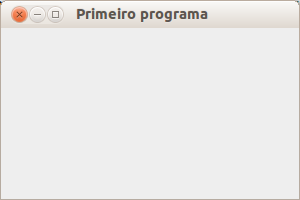
\includegraphics[0.5]{images/primeiro_programa}
    \caption{Resultado do PrimeiroPrograma.java}
    \label{figRotulo}
  \end{figure}
\end{frame}{}

\subsection{JDialog}
\begin{frame}{Nosso primeiro programa}{JDialog}
\end{frame}{}

\subsection{JApplet}
\begin{frame}{Nosso primeiro programa}{Top-Level Containers}{JApplet}
\end{frame}{}


\section{Menu e ToolBar}
\begin{frame}{Menu e ToolBar}{}
\end{frame}{}

\subsection{JToolBar}
\begin{frame}{Menu e ToolBar}{JToolBar}
\end{frame}{}


\section{Layouts}
\begin{frame}{Layouts}{}
\end{frame}{}

\subsection{FlowLayout}
\begin{frame}{Layouts}{FlowLayout}
\end{frame}{}

\subsection{GridLayout}
\begin{frame}{Layouts}{GridLayout}
\end{frame}{}

\subsection{BorderLayout}
\begin{frame}{Layouts}{BorderLayout}
\end{frame}{}

\subsection{BoxLayout}
\begin{frame}{Layouts}{BoxLayout}
\end{frame}{}


\section{Caixas de Diálogo}
\begin{frame}{Caixas de Diálogo}{}
\end{frame}{}

\subsection{JDialog}
\begin{frame}{Caixas de Diálogo}{JDialog}
\end{frame}{}
\subsection{Criando uma caixa de mensagem}
\begin{frame}{Caixas de Diálogo}{Criando uma caixa de mensagem}
\end{frame}{}

\subsection{JFileChooser}
\begin{frame}{Caixas de Diálogo}{JFileChooser}
\end{frame}{}

\subsection{JColorChooser}
\begin{frame}{Caixas de Diálogo}{JColorChooser}
\end{frame}{}


\section{Componentes básicos}
\begin{frame}{Componentes básicos}{}
\end{frame}{}

\subsection{Componentes de Texto}
\begin{frame}{Componentes básicos}{Componentes de Texto}
\end{frame}{}

\subsubsection{TextField}
\begin{frame}{Componentes básicos}{Componentes de Texto}{TextField}
\end{frame}{}

\subsubsection{FormattedTextField}
\begin{frame}{Componentes básicos}{Componentes de Texto}{FormattedTextField}
\end{frame}{}

\subsubsection{PasswordField}
\begin{frame}{Componentes básicos}{Componentes de Texto}{PasswordField}
\end{frame}{}
\subsubsection{TextArea}
\begin{frame}{Componentes básicos}{Componentes de Texto}{TextArea}
\end{frame}{}
\subsubsection{Usando HTML em Componentes Swing}
\begin{frame}{Componentes básicos}{Componentes de Texto}{Usando HTML em Componentes Swing}
\end{frame}{}
\subsection{Bordas}
\begin{frame}{Componentes básicos}{Bordas}
\end{frame}{}
\subsection{Ícones e Imagens}
\begin{frame}{Componentes básicos}{Ícones e Imagens}
\end{frame}{}
\subsection{Tabelas}
\begin{frame}{Componentes básicos}{Tabelas}
\end{frame}{}
\subsubsection{JTable}
\begin{frame}{Componentes básicos}{Tabelas}{JTable}
\end{frame}{}
\subsubsection{Criando uma tabela simples}
\begin{frame}{Componentes básicos}{Tabelas}{Criando uma tabela simples}
\end{frame}{}
\subsection{Painel de rolagem}
\begin{frame}{Componentes básicos}{Painel de rolagem}
\end{frame}{}
\subsubsection{JScrollPane}
\begin{frame}{Componentes básicos}{Painel de rolagem}{JScrollPane}
\end{frame}{}
\subsection{Botões}
\begin{frame}{Componentes básicos}{Botões}
\end{frame}{}
\subsubsection{JButton}
\begin{frame}{Componentes básicos}{Botões}{JButton}
\end{frame}{}
\subsubsection{JCheckBox}
\begin{frame}{Componentes básicos}{Botões}{JCheckBox}
\end{frame}{}
\subsubsection{JRadioButton}
\begin{frame}{Componentes básicos}{Botões}{JRadioButton}
\end{frame}{}
\subsubsection{JMenuItem}
\begin{frame}{Componentes básicos}{Botões}{JMenuItem}
\end{frame}{}
\subsubsection{JCheckBoxMenuItem}
\begin{frame}{Componentes básicos}{Botões}{JCheckBoxMenuItem}
\end{frame}{}
\subsubsection{JRadioButtonMenuItem}
\begin{frame}{Componentes básicos}{Botões}{JRadioButtonMenuItem}
\end{frame}{}
\subsubsection{JToggleButton}
\begin{frame}{Componentes básicos}{Botões}{JToggleButton}
\end{frame}{}
\subsection{Outros}
\begin{frame}{Componentes básicos}{Outros}
\end{frame}{}
\subsubsection{ProgressBar}
\begin{frame}{Componentes básicos}{Outros}{ProgressBar}
\end{frame}{}
\subsubsection{Spinner}
\begin{frame}{Componentes básicos}{Outros}{Spinner}
\end{frame}{}
\subsubsection{JList}
\begin{frame}{Componentes básicos}{Outros}{JList}
\end{frame}{}
\section{Desenhando com o Swing}
\begin{frame}{Desenhando com o Swing}{}
\end{frame}{}
\subsection{Pontos}
\begin{frame}{Desenhando com o Swing}{Pontos}
\end{frame}{}
\subsection{Linhas}
\begin{frame}{Desenhando com o Swing}{Linhas}
\end{frame}{}
\subsection{Figuras Geometricas}
\begin{frame}{Desenhando com o Swing}{Figuras Geometricas}
\end{frame}{}
\subsection{Colorindo}
\begin{frame}{Desenhando com o Swing}{Colorindo}
\end{frame}{}
\section{Eventos}
\begin{frame}{Eventos}{}
\end{frame}{}
\subsection{ActionEvent}
\begin{frame}{Eventos}{ActionEvent}
\end{frame}{}
\section{Exemplos}
\begin{frame}{Exemplos}{}
\end{frame}{}
\subsection{Tetrix}
\begin{frame}{Exemplos}{Tetrix}
\end{frame}{}
\subsection{Puzzle}
\begin{frame}{Exemplos}{Puzzle}
\end{frame}{}
\section{Referências}
\begin{frame}{Referências}{}
\begin{itemize}
\item Window Builder - https://www.eclipse.org/windowbuilder/
\item Swing tutorial - http://www.tutorialspoint.com/swing/
\item Swing tutorial(verboso) - http://www.wikihow.com/Create-a-Swing-GUI-in-Java
\item Swing tuto mais completo - http://zetcode.com/tutorials/javaswingtutorial/
\item Swing oficial - http://docs.oracle.com/javase/tutorial/uiswing/components/
\item Swing oficial - http://docs.oracle.com/javase/tutorial/uiswing/
\item Swing javadoc - http://docs.oracle.com/javase/7/docs/api/javax/swing/package-summary.html
\end{itemize}
\end{frame}
\end{document}